%!TEX root = ../msc_thesis.tex

\chapter{Artificial Neural Networks}
\label{ch:ann}

%%%%%%%%%%%%%%%%%%%%%%%%%%%%%%%%%%%%%%%%%%%%%%%%%%%%%%%%%%%%%%%%%%%%%%%%%%%%%%%%%%%%%%%%%%
%%%%%%%%%%%%%%%%%%%%%%%%%%%%%%%%%%%%%%%%%%%%%%%%%%%%%%%%%%%%%%%%%%%%%%%%%%%%%%%%%%%%%%%%%%
%%% ANNs
%%%%%%%%%%%%%%%%%%%%%%%%%%%%%%%%%%%%%%%%%%%%%%%%%%%%%%%%%%%%%%%%%%%%%%%%%%%%%%%%%%%%%%%%%%
%%%%%%%%%%%%%%%%%%%%%%%%%%%%%%%%%%%%%%%%%%%%%%%%%%%%%%%%%%%%%%%%%%%%%%%%%%%%%%%%%%%%%%%%%%

In Chapter \ref{ch:machine_learning} it was mentioned that in supervised learning there is a response variable $\boldsymbol{y} \in \mathbb{R}^n$ and a data matrix $\boldsymbol{X} \in \mathbb{R}^{n \times p}$. It is assumed that there exists a relationship between $\boldsymbol{y}$ and $\boldsymbol{X}$ such that
$\boldsymbol{y} = f(\boldsymbol{X}) + \boldsymbol{\varepsilon}$,
with $f$ being a fixed but unknown function. Since $f$ is unknown, it is estimated with a function $\hat{f}$ that is chosen from a parameterized family of functions $\mathcal{F}_{\boldsymbol{\theta}}$. Artificial neural networks (ANNs) belong to one of the families from which $\mathcal{F}_{\boldsymbol{\theta}}$ can be chosen. In this chapter, two types of ANNs will be studied, feed-forward neural networks and convolutional neural networks (CNNs).

\section{Artificial Neural Networks}

The most basic, and perhaps the best known, type of ANN is the feed-forward neural network, also widely called multilayer perceptron (MLP). This concept will be first introduced in the frequentist framework and then they will be explained in the Bayesian framework.

To illustrate the multilayer perceptron, consider a simple example: a researcher wants to model a continuous variable $\boldsymbol{y}$ from a single feature $\boldsymbol{x}$. A very simple model would be a linear regression, in which each observation $i$ is modeled as $y_i = \theta_0 + \theta_1 x_i$, with $\theta_0$ and $\theta_1$. ANNs go further and take non-linear transformations of this linear predictor with some function $\sigma(\cdot)$,
such that $y_i = \theta_0^{[1]} +  \sum_{j = 1}^m \theta_j^{[1]} \sigma \left( \theta_0^{[0]} + \theta_j^{[0]} x_i \right)$,
where $m$ is a tuning hyperparameter previously chosen.
Function $\sigma(\cdot)$ is called the \textbf{activation function}, and is very often chosen to be the logistic sigmoid function $\sigma(x) = (1 + e^{-x})^{-1}$
or the hyperbolic tangent $\sigma(x) = \tanh(x)$.
%The values of parameters $\theta_k^{[0]}$ and $\theta_k^{[1]}$ for $k \in \left\{ 0, \ldots, m \right\}$ are also chosen to minimize certain error function.

Figure \ref{fig:theory_ANN_diagram_01} shows these relationships in a graphic way for a model with $m = 3$ and where $a_{k, i}$ is defined as $a_{k, i} = \sigma \left( \theta_0^{[0]} + \theta_k^{[0]} x_i \right)$ for $k \in \left\{ 1, 2, 3 \right\}$.
For simplicity, this image does not explicitly show the parameters $\theta_0^{[0]}$ and $\theta_0^{[1]}$, which are called the \textbf{bias} parameters.

\begin{figure}[H]
    \centering
    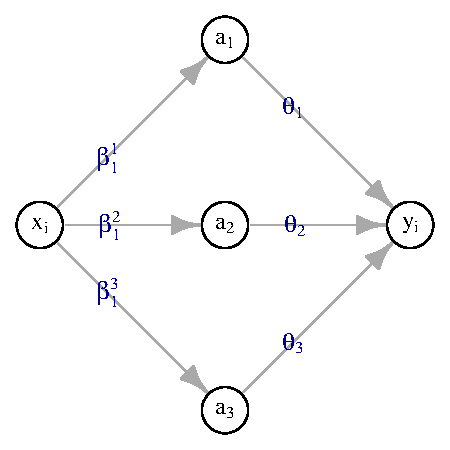
\includegraphics[width=0.5\textwidth]{plot_ANN_01.pdf}
    \caption{Diagram of a multilayer perceptron with $m = 3$.}
    \label{fig:theory_ANN_diagram_01}
\end{figure}

If the response variable $\boldsymbol{y}$ happened to be a binary variable, then one last transformation needs to be applied to map the model to the $\left[0, 1\right]$ interval and model $\boldsymbol{y}$ as a probability, just as in logistic regression. In the case of a binary response variable, $y_i$ could be written as
\begin{equation}
  y_i =
  \phi \left( \theta_0^{[1]} +  \sum_{j = 1}^m \theta_j^{[1]} \sigma \left( \theta_0^{[0]} + \theta_j^{[0]} x_i \right) \right) =
  \phi \left( \theta_0^{[1]} +  \sum_{j = 1}^m \theta_j^{[1]} a_{j,i} \right),
\end{equation}
with $\phi(\cdot)$ the logistic sigmoid function to map from $\mathbb{R}$ to $\left[ 0, 1 \right]$. The choice of function $\phi(\cdot)$ depends on the nature of the response variable. In the case of a continuous response variable, $\phi(\cdot)$ is the identity function; in a binary classification problem, it could be the logistic sigmoid function; and in the case of a classification problem with more than two categories, a softmax function could be used.

A more complex model can be created by taking linear combinations of non-linear functions of the previous result. Let
\begin{equation}
a_{k,i}^{[1]} = \sigma^{[1]} \left( \theta_{0}^{[1]} + \theta_k^{[0]} x_i \right)
\end{equation}
for $k \in \left\{ 1, \ldots, m \right\}$ and
\begin{equation}
  a_{k,i}^{[2]} = \sigma^{[2]} \left(  \theta_{0,k}^{[1]} + \sum_{j = 1}^m \theta_{j,k}^{[1]} a_{j,1}^{[0]}  \right)
\end{equation}for $k \in \left\{ 1, \ldots, r \right\}$.

Then
\begin{equation}
  y_i = \theta_0^{[2]} + \sum_{j = 1}^r \theta_j^{[2]} a_{j,i}^{[2]}
\end{equation}
where $r$, like $m$, is chosen beforehand. The values $m$ and $r$ are called the number of nodes or units of each layer. This is a deeper model than the last one because it has more layers. Notice that there are two different activation functions $\sigma^{[1]}(\cdot)$ and $\sigma^{[2]}(\cdot)$. Each layer can have a different function. The first one could be a sigmoid function and the second one a hyperbolic tangent, or vice versa, or they could both be the same function.

Figure \ref{fig:theory_ANN_diagram_02} shows this graphically with $m = 3$ and $r = 2$. Layers corresponding to $a_{k,i}^{[1]}$ for $k \in \left\{ 1, \ldots, m \right\}$ and $a_{k,i}^{[2]}$ for $k \in \left\{ 1, \ldots, r \right\}$ are called the \textbf{hidden layers}.
Figure \ref{fig:theory_ANN_diagram_01} shows a multilayer perceptron with one hidden layer, and figure \ref{fig:theory_ANN_diagram_02} shows a multilayer perceptron with two hidden layers.

\begin{figure}[H]
    \centering
    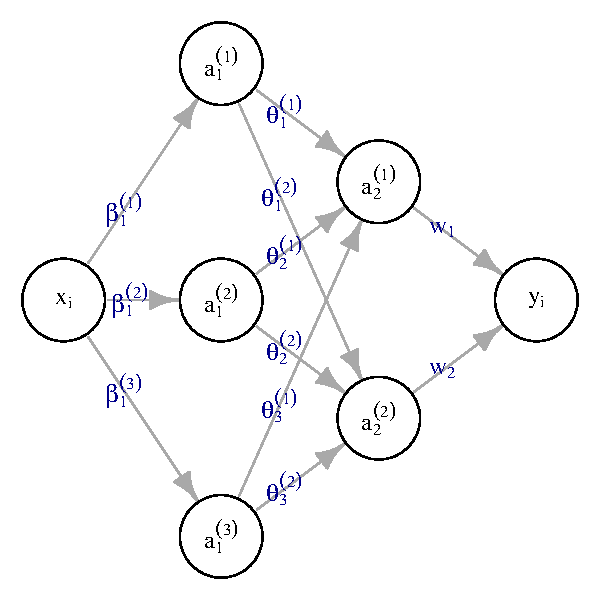
\includegraphics[width=0.6\textwidth]{plot_ANN_02.pdf}
    \caption{Diagram of a multilayer perceptron with two hidden layers, $m = 3$ and $r = 2$.}
    \label{fig:theory_ANN_diagram_02}
\end{figure}

After these two introductory examples of MLPs, they can be defined in a more formal and general fashion.
As before, $\boldsymbol{y}$ denotes the response variable, and $y_i$ denotes the $i$-th element of $\boldsymbol{y}$.
Once again, $\boldsymbol{X} \in \mathbb{R}^{n \times p}$ denotes the data matrix; $\boldsymbol{x}_i \in \mathbb{R}^p$ denotes the $i$-th row in $\boldsymbol{X}$, representing the values of the features for the $i$-th element in the data; $\boldsymbol{x}^{(k)} \in \mathbb{R}^n$ denotes the $k$-th column in $\boldsymbol{X}$; and $x_i^{(k)}$ denotes the $k$-th column-wise element and the $i$-th row-wise element.

A multilayer perceptron can have any integer number of layers, and this number will be denoted by $L$. The number of nodes of each layer $l$ will be denoted by $n^{[l]}$. And the activation function for each layer $l$ will be denoted by $\sigma^{[l]}(\cdot)$, for $l \in \left\{ 1, \ldots, L \right\}$. The activation function for the last layer will be denoted by $\phi(\cdot)$, as in the binary classification example. The parameter that connects the $j$-th node from the $(l-1)$-th layer with the $k$-th node in the $l$-th layer is denoted by $\theta_{j,k}^{[l]}$ and, as before, $a_{k,i}^{[l]}$ denotes the result of the activation function corresponding to the $l$-th layer and the $i$-th observation, for $k \in \left\{ 1, \ldots, n^{[l]} \right\}$; where $\theta_{0,k}^{[l]}$ is the bias term of the $k$-th node in the $l$-th layer. This notation can be summarized as follows,
\begin{equation}
  \label{eq:ann_act_funct_def}
  a_{k,i}^{[l]} = \sigma^{[l]} \left( \theta_{0,k}^{[l-1]} + \sum_{j = 1}^{n^{[l-1]}} \theta_{j,k}^{[l-1]} a_{j,i}^{[l-1]} \right)
\end{equation}
for $k \in \left\{ 1, \ldots, n^{[l]} \right\}$, $j \in \left\{ 1, \ldots, n^{[l-1]} \right\}$, $l \in \left\{ 1, \ldots, L \right\}$ and $i \in \left\{ 1, \ldots, n \right\}$.

To be consistent, $a_{k,i}^{[0]}$ is defined as $x_i^{[k]}$, hence, $\boldsymbol{a}_{k}^{[0]} = \boldsymbol{x}^{(k)} \in \mathbb{R}^n$; and $a_{0,i}^{[0]} = 1$ for all $i \in \left\{ 1, \ldots, n \right\}$, so $\boldsymbol{a}_{0}^{[0]}$ is a vector of ones of dimension $n$ and $n^{[0]}$ is the number of features, i.e., $n^{[0]} = p$.

In general, a feed-forward neural network or multilayer perceptron with $L$ hidden layers is such that
\begin{equation}
  y_i = \phi \left( \theta_{0,1}^{[L]} +  \sum_{j = 1}^{n^{[L]}} \theta_{j,1}^{[L]} a_{k,i}^{[L]} \right),
\end{equation}
where equation \eqref{eq:ann_act_funct_def} must be held. As a way to summarize the whole notation, a multilayer perceptron with parameters $\boldsymbol{\Theta}$ and data matrix $\boldsymbol{X}$ will be denoted as $\mathrm{MLP} \left(\boldsymbol{X}, \boldsymbol{\Theta} \right)$, where parameter $\boldsymbol{\Theta}$ is a general way to refer to all parameters $\theta_{j,k}^{[l]}$ for $k \in \left\{ 1, \ldots, n^{[l]} \right\}$, $j \in \left\{ 1, \ldots, n^{[l-1]} \right\}$ and $l \in \left\{ 1, \ldots, L \right\}$.

Figure \ref{fig:theory_ANN_diagram_03} shows an example of an architecture with 2 hidden layers ($L = 2$), 4 features ($p = n^{[0]} = 4$), 3 nodes in the first hidden layer ($n^{[1]} = 3$) and 4 nodes in the second hidden layer ($n^{[2]} = 4$).

\begin{figure}[H]
    \centering
    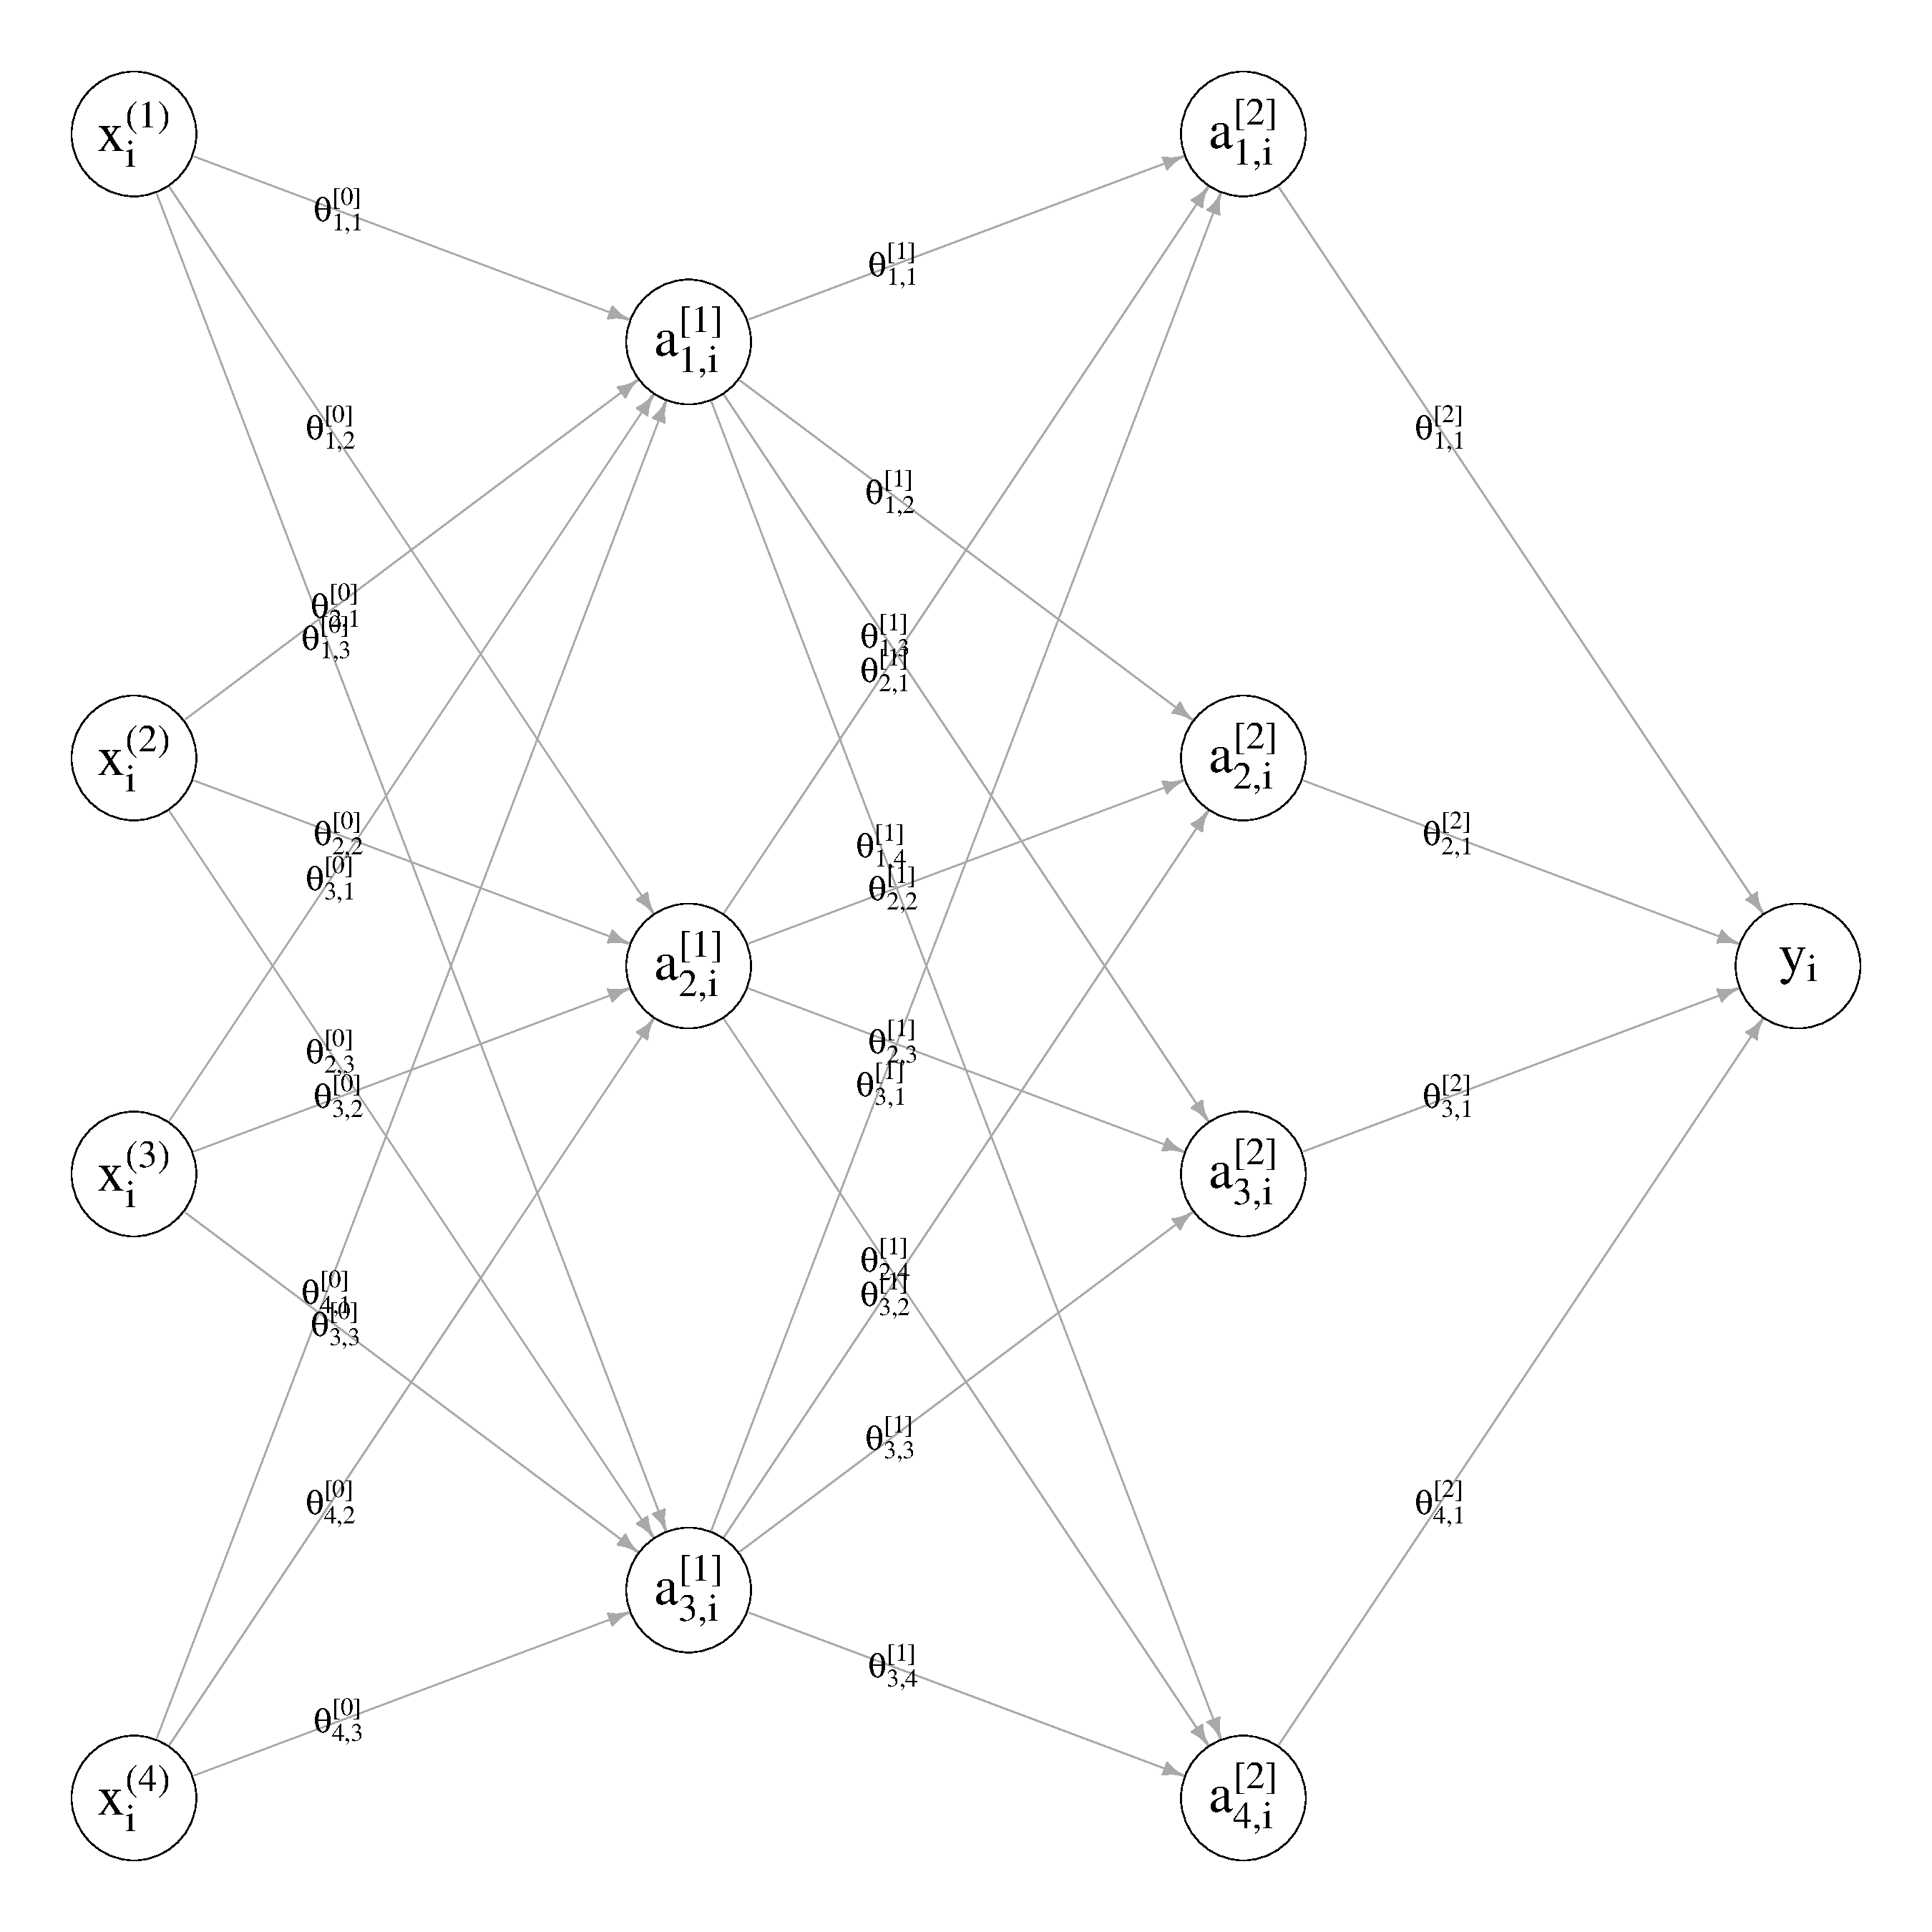
\includegraphics[width=0.95\textwidth]{plot_ANN_03.pdf}
    \caption{Diagram of a multilayer perceptron with two hidden layers using the general notation with $L = 2$, $p = n^{[0]} = 4$, $n^{[1]} = 3$ and $n^{[2]} = 4$.}
    \label{fig:theory_ANN_diagram_03}
\end{figure}

In the ANN literature, the most common approach to estimate the network parameters is the loss function minimization approach. In most cases, this approach results in the same estimate as in the maximum likelihood approach because of the way in which loss functions are defined. Hyperparameters, such as the number of layers and the number of neurons, are usually chosen by a cross-validation scheme, or with a validation set.

As mentioned in Chapter \ref{ch:machine_learning}, when the response variable is continuous, the quadratic loss is often used, and it is equivalent to the maximization of a Gaussian likelihood function. In the case of a binary classification problem, the binary entropy loss defined in \eqref{eq:logistic_example_loss_function}, is usually used, and it is equivalent to maximizing the likelihood of independent Bernoulli response variables.

In the case of a multiple classification problem, the cross-entropy loss is extended to accommodate for more classes using the same maximum likelihood idea. In a $K$ class classification problem, the loss is defined as
\begin{equation}
  L(\boldsymbol{\Theta}) = - \sum_{i = 1}^n \left[ \sum_{j = 1}^K y_{i,j} \log{\left( \hat{y}_{i,j} \right)}  \right]
\end{equation}
where $y_{i,j} = 1$ if the $i$-th training point belongs to the $j$-th class and $\hat{y}_{i,j}$ is the model's predicted probability of the $i$-th training point belonging to the $j$-th class.

In the Bayesian approach, the idea is the same as was explained in Chapter \ref{ch:machine_learning}. Each of the parameters is assigned a prior distribution and the response variable $\boldsymbol{y}$ is assumed to be generated by a probabilistic model with unknown parameters. The latter are assumed to be random variables as well, to be able to represent the uncertainty on their values. For example, in the continuous case, a Gaussian conditional distribution to $\boldsymbol{y}$ can be assigned, such that
\begin{equation}
  \boldsymbol{y} | \boldsymbol{\Theta}, \boldsymbol{X} \sim \normaldist{\mathrm{MLP}(\boldsymbol{X}, \boldsymbol{\Theta})}{\sigma^2}
\end{equation}
where $\mathrm{MLP}(\boldsymbol{X}, \boldsymbol{\Theta})$ denotes the architecture of a multilayer perceptron with parameters $\boldsymbol{\Theta}$ and data matrix $\boldsymbol{X}$. As was mentioned before, since the $\boldsymbol{\Theta}$ parameters can be any real value, it is also common to assign a Gaussian distribution to them, so that the prior distribution is such that
\begin{equation}
  \theta_{i,k}^{[l]} \sim \normaldist{\mu_{i,k}^{[l]}}{\sigma_{i,k}^{[l]}}.
\end{equation}

Bayes' theorem is used to update the knowledge about the parameters given the data in the following way
\begin{equation}
  \prob{\boldsymbol{\Theta} | \boldsymbol{X}, \boldsymbol{y}} = \frac{\prob{\boldsymbol{y} | \boldsymbol{\Theta}, \boldsymbol{X}} \prob{\boldsymbol{\Theta} | \boldsymbol{X}}}{\prob{\boldsymbol{y} | \boldsymbol{X}}}.
\end{equation}

In the example above, $\prob{\boldsymbol{y} | \boldsymbol{\Theta}, \boldsymbol{X}}$ and $\prob{\boldsymbol{\Theta} | \boldsymbol{X}}$ are the joint density functions of Gaussian random variables with their corresponding parameter values. To make predictions, the posterior predictive distribution defined in equation \eqref{eq:post_pred_dist} is used.

As mentioned in Chapter \ref{ch:variational_inference}, complex Bayesian models such as Bayesian ANN can be intractable or too slow for typical numerical approaches such as MCMC. The reason is that ANNs tend to have a high-dimensional parameter vector, for which off-the-shelf MCMC approaches struggle to reach stationarity of the Markov Chain. In this sense, dropout, the stochastic regularization technique mentioned in Chapter \ref{ch:machine_learning}, can be seen as a variational approximation to a Bayesian neural network and to a deep Gaussian process \cite{gal2015dropout, gal2015dropout1, gal2015bayesian, gal2015modern}. Particularly, applying dropout before each weight layer in a neural network with arbitrary depth is mathematically equivalent to a variational approximation that minimizes the KL divergence to the posterior distribution of a Bayesian neural network. This approximation includes convolutional neural networks, presented in the next section.



%%%%%%%%%%%%%%%%%%%%%%%%%%%%%%%%%%%%%%%%%%%%%%%%%%%%%%%%%%%%%%%%%%%%%%%%%%%%%%%%%%%%%%%%%%
%%%%%%%%%%%%%%%%%%%%%%%%%%%%%%%%%%%%%%%%%%%%%%%%%%%%%%%%%%%%%%%%%%%%%%%%%%%%%%%%%%%%%%%%%%
%%% CNNs
%%%%%%%%%%%%%%%%%%%%%%%%%%%%%%%%%%%%%%%%%%%%%%%%%%%%%%%%%%%%%%%%%%%%%%%%%%%%%%%%%%%%%%%%%%
%%%%%%%%%%%%%%%%%%%%%%%%%%%%%%%%%%%%%%%%%%%%%%%%%%%%%%%%%%%%%%%%%%%%%%%%%%%%%%%%%%%%%%%%%%

\section{Convolutional Neural Networks}

Convolutional Neural Networks (CNNs) are neural networks with a particular architecture and are widely used in computer vision problems, such as image classification or object detection in videos. They were introduced by \citeauthor{lecun1989generalization} in \citeyear{lecun1989generalization} as a way to constrain the number of parameters needed to perform automatic image classification \cite{lecun1989generalization}. The main idea is that in images, pixels close to each other tend to be similar, whereas pixels far away from each other tend to be different. This notion of proximity is used by CNN's architecture, and leverages three concepts: sparse interactions, parameter sharing and equivariant representations \cite[p.~335]{bengio2015deep}.

\begin{itemize}
  \item Sparse interactions: In MLPs, every unit is connected to all other units in the next layer, but in CNNs, only few units are connected to other few of units. This means fewer parameters and, hence, less memory usage and faster computation.
  \item Parameter sharing: Different units share the same set of parameters. The same convolution is used many times in the image and, thus, the number of parameters is further reduced.
  \item Equivariant representations: The architecture of CNNs provides equivariance in translations, meaning that if the input is changed, the output is changed in the same fashion. For example: in an image, if an object is moved in the input, its representation will be moved in the same way in the output.
\end{itemize}

\subsection{Convolution operation}

The base of CNNs is the convolution operation. This is a general operation, but for this work, it will be described assuming that the input is a digital image. This image is represented as an $m \times n$ matrix $\boldsymbol{I}$, where $I_{i,j}$ represents the pixel in the $i$-th row and $j$-th column as such
\begin{equation}
  \boldsymbol{I} =
    \begin{bmatrix}
      I_{1,1} & I_{1,2} & I_{1,3} & \dots  & I_{1,n} \\
      I_{2,1} & I_{2,2} & I_{2,3} & \dots  & I_{2,n} \\
      \vdots & \vdots & \vdots & \ddots & \vdots \\
      I_{m,1} & I_{m,2} & I_{m,3} & \dots  & I_{m,n}
    \end{bmatrix}.
\end{equation}

The convolution operation uses another matrix called a \textbf{filter} or a \textbf{kernel}, with dimensions $p \times r$, where $p < m$ and $r < n$. This means that the kernel matrix must be of a lower dimension than the image $\boldsymbol{I}$. The filter matrix is denoted by $\boldsymbol{K}$ as
\begin{equation}
  \boldsymbol{K} =
    \begin{bmatrix}
      \theta_{1,1} & \theta_{1,2} & \theta_{1,3} & \dots  & \theta_{1,q} \\
      \theta_{2,1} & \theta_{2,2} & \theta_{2,3} & \dots  & \theta_{2,q} \\
      \vdots & \vdots & \vdots & \ddots & \vdots \\
      \theta_{p,1} & \theta_{p,2} & \theta_{p,3} & \dots  & \theta_{p,q}
    \end{bmatrix}.
\end{equation}

The convolution operation between $\boldsymbol{I}$ and $\boldsymbol{K}$ is denoted as $\boldsymbol{I} * \boldsymbol{K}$, and its result is another matrix $\boldsymbol{S}$. Each element of $\boldsymbol{S}$ is defined as
\begin{equation}
  \label{eq:2d_conv_def}
  S_{i,j} = (\boldsymbol{I} * \boldsymbol{K})_{i,j} = \sum_{k} \sum_{l} I_{i+k-1,j+l-1} K_{k, l}.
\end{equation}

An example of this is shown in figure \ref{fig:conv_example}, in which $\boldsymbol{I}$ is a $7 \times 7$ image matrix and the kernel $\boldsymbol{K}$ is a $3 \times 3$ matrix. The result is a $5 \times 5$ matrix in which each element is computed using equation \eqref{eq:2d_conv_def}. For instance, the element on the first row and fourth column of $\boldsymbol{S}$, that is, $S_{1,4}$ is computed as
\begin{equation}
  \begin{split}
      S_{1,4} & =
      \sum_{k=1}^3 \sum_{l=1}^3 I_{1+k-1,4+l-1} K_{k, l} \\
      & = I_{1,4}K_{1,1} + I_{1,5}K_{1,2} + I_{1,6}K_{1,3} \\
      & + I_{2,4}K_{2,1} + I_{2,5}K_{2,2} + I_{2,6}K_{2,3} \\
      & + I_{3,4}K_{3,1} + I_{3,5}K_{3,2} + I_{3,6}K_{3,3} \\
      & = ( 1 \times 1 ) + ( 0 \times 0 ) + ( 0 \times 1 ) \\
      & + ( 1 \times 0 ) + ( 1 \times 1 ) + ( 0 \times 0 ) \\
      & + ( 1 \times 1 ) + ( 1 \times 0 ) + ( 1 \times 1 ) \\
      & = 4.
  \end{split}
\end{equation}
The rest of the elements are computed in a similar way. It should be noted that the resulting matrix is smaller than the original image matrix.

\begin{figure}[H]
    \centering
    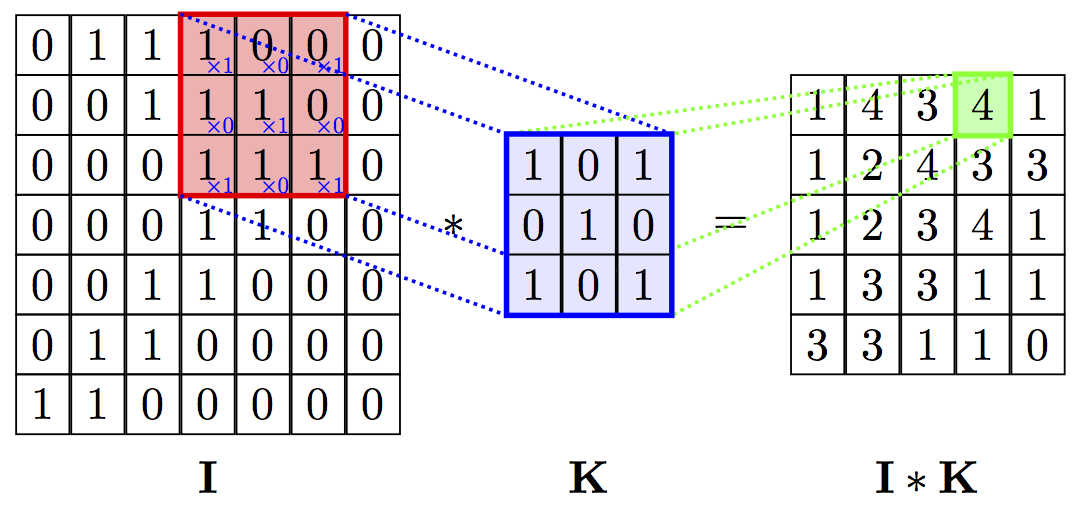
\includegraphics[width=0.9\textwidth]{convolution_example.png}
    \caption{Example of a convolution operation. Source: \url{https://github.com/PetarV-/TikZ}}
    \label{fig:conv_example}
\end{figure}

The convolution kernel in the example only has 9 parameters which are used by the whole image matrix, and these parameters are usually estimated with data.

An image classification problem could be solved by turning the input image into a long vector, but then this would be fed to a fully connected layer, which would mean that a large number of parameters would have to be fitted. This is one of the reasons convolutions are used: instead of estimating a large number of parameters, the convolution operation needs a small number of parameters (9 in the case of the example) to be estimated. Additionally, the convolution operation takes into account the topology of the image input, which has a very local structure \cite{lecun1998gradient}.

\subsection{Pooling}

When using CNNs, a pooling layer is also usually added after each convolutional layer. This pooling layer summarizes adjacent pixels, and it is used because it helps to achieve invariance and reduce the image of the output so that there are fewer parameters in the next layers \cite{bengio2015deep}. A very commonly used pooling function is \textbf{max pooling}, which returns the maximum value of a neighborhood of pixels. An example of max pooling is shown in figure \ref{fig:max_pool_example} for a $4 \times 4$ matrix, resulting in a $2 \times 2$ matrix after the function is applied.

\begin{figure}[H]
    \centering
    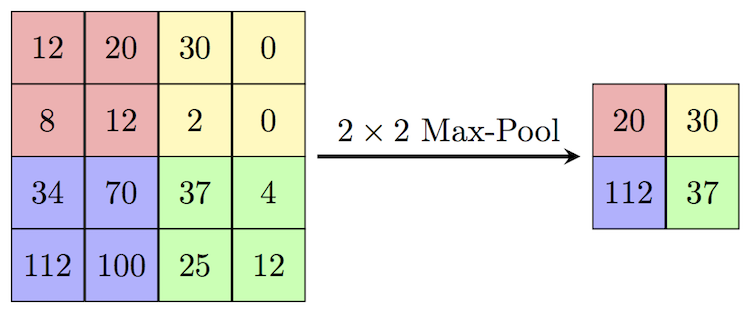
\includegraphics[width=0.6\textwidth]{max_pool_example.png}
    \caption{Example of max pooling function. Source: \url{https://computersciencewiki.org/index.php/File:MaxpoolSample2.png}}
    \label{fig:max_pool_example}
\end{figure}


\subsection{Architecture example}

To illustrate how all these concepts are put together, an example of an architecture that is very commonly used in image classification problems is discussed. This architecture is called the \textbf{LeNet architecture}, and it was introduced by \citeauthor{lecun1998gradient} in \citeyear{lecun1998gradient} for a digit classification problem \cite{lecun1998gradient}. The architecture assumes a grayscale input image of $32 \times 32$ pixels, which is then fed to 6 convolutional filters of size $5 \times 5$, each followed by an activation function and a $2 \times 2$ max pooling layer, then 16 convolutional filters of size $5 \times 5$, each with their corresponding activation functions and then the $2 \times 2$ max pooling layer, followed by two fully connected layers of sizes 120 and 84, and finally a softmax transformation to map to the 10 digit classification problem probabilities.

\begin{figure}[H]
    \centering
    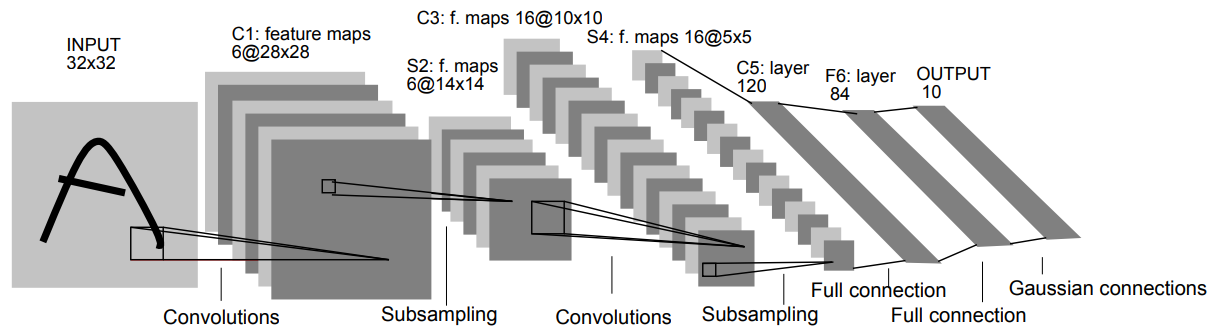
\includegraphics[width=\textwidth]{lenet.png}
    \caption{LeNet architecture (picture taken from \cite{lecun1998gradient}). The feature maps correspond to the convolutional filters and the subsampling refers to max pooling.}
    \label{fig:lenet_architecture}
\end{figure}

This chapter described the basic idea of ANNs and CNNs. Chapter \ref{ch:active_learning} will discuss the Active Learning methodology and Chapter \ref{ch:results} will present numerical experiments in which the ideas of the previous chapters are used together and compared with each other.
